% 2011 年浙江卷理科第 21 题：抛物线 C1: x^2=y 与圆 C2: x^2+(y-4)^2=1。
% 来源 PDF：普通高考/2011/2011浙江理.pdf，SHA-256 0239778f574bc3ce6d7aca5024aa6333f80d131abaf699f79c46472394f8cd65。
% 原页：第 2 页第 2 栏，书页码 710。示意。
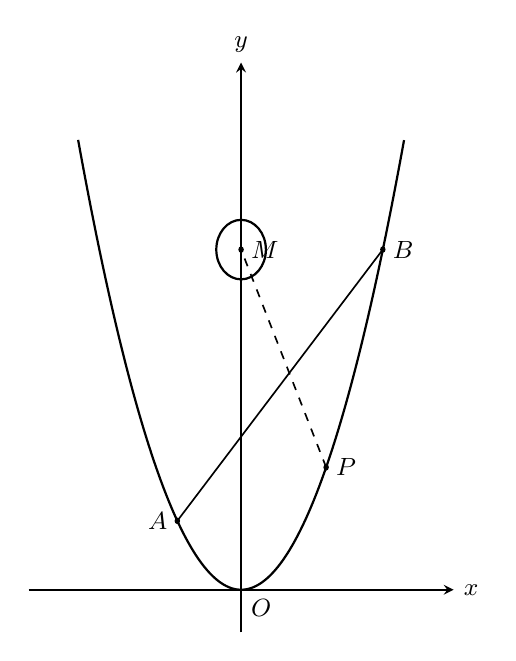
\begin{tikzpicture}[>=stealth, semithick, font=\small, scale=0.9, yscale=1.2]
  \draw[->] (-3,0)--(3,0) node[right] {$x$};
  \draw[->] (0,-0.5)--(0,6.2) node[above] {$y$};
  \draw[thick, domain=-2.3:2.3, samples=120] plot (\x, {\x*\x});
  \draw[thick] (0,4) circle (0.35);
  \fill (0,4) circle (1.1pt) node[right] {$M$};
  \coordinate (P) at (1.2,1.44);
  \fill (P) circle (1.1pt) node[right] {$P$};
  \coordinate (A) at (-0.9,0.81);
  \coordinate (B) at (2.0,4.0);
  \fill (A) circle (1.1pt) node[left] {$A$};
  \fill (B) circle (1.1pt) node[right] {$B$};
  \draw (A)--(B);
  \draw[dashed] (P)--(0,4);
  \node[below right] at (0,0) {$O$};
\end{tikzpicture}
